\textbf{Spørgsmål}\\
Med udgangspunkt i eksperiment ”Michaelis-Menten DTU” skal du redegøre for, hvorledes man i praksis kan bestemme $K_M$ og $v_{max}$ for en enzymkatalyseret reaktion.

I din gennemgang kan du gøre brug af nedenstående stikord. 

I din besvarelse skal bilagene inddrages.

\vspace{.5cm}
\textbf{Stikord}: Aminosyrer, proteiner, enzymer, hæmning, reaktionshastighed, reaktionsorden, temperatur og katalysatorer.

\section*{Synopsis}
\subsection{Enzymer}
Enzymer er ligesom proteiner bygget af aminosyrekæder. 
Disse kæder kan være foldet på forskellig vis (se 168 A).
Enten kan de være foldet til $\alpha$-helixer eller i $\beta$-foldebladsstrukturer.

\subsection{Enzymers virkemåde og reaktionshastighed}
Enzymer fungerer som katalysatorer i reaktioner. 
I en proces hvor de skal omdanne et stof $S$ (kaldet substratet) til et stof $P$ (produktet), laver enzymet $E$ først en reaktion med $S$ således at de nu sidder sammen i et enzym-substrat-kompleks, $ES$ (se side 174 A).
Enzym-substrat-komplekset kan da skilles ad igen over til produktet og enzymet.
Dette giver anledning til et reaktionskema på følgende form:
$$ S + E \rightleftharpoons ES \rightleftharpoons P + E  $$
Til at starte med har vi dog intet produkt, hvorfor reaktionen fra $P$ til $SE$ er så langsom at den kan ignoreres:
$$ S + E \overset{k_1}{\underset{k_{\text{-}1}}{\rightleftharpoons}} ES \overset{k_2}{\rightarrow} P + E  $$
Ved reaktionspilene er noteret deres hastighedskonstanter. 
Vi kan da beskrive hvor reaktionshastigheder der beskriver hvor hurtigt $ES$ dannes/opbruges. 
ved:
$$\text{Dannelse: } k_1 \cdot [S] \cdot [E]$$
$$\text{Opbrugelse: } k_{\text{-}1} \cdot [ES] + k_2 \cdot [ES]=[ES]\cdot (k_{\text{-}1} + k_2)$$
Forholdscist hurtigt vil der indstilles en ligevægt hvor stofmængden af $ES$ er konstant. 
Her vil det naturligvis gælde at $ES$ dannes og opbruges lige hurtigt, hvorfor de to ligniger fra før må være lig hinanden:
$$ k_1 \cdot [S] \cdot [E] = [ES]\cdot (k_{\text{-}1} + k_2) $$
Ved omskrivning får vi:
$$ \dfrac{[S] \cdot [E]}{[ES]} = \dfrac{k_{\text{-}1} + k_2}{k_1 } \overset{\text{def}}{=} K_M $$
Ved omskrivningen definerer vi en ny størrelse $K_M$, som kaldes Michalis-konstanten.

\subsubsection{Udledning af Michalis-Menten ligningen}
Michalis-Menten ligningen siger at $ v = v_{max} \cdot \dfrac{[S]}{K_M + [S]} $. hvor $v$ er hastigheden hvormed $P$ dannes og $v_{max}$ er den maksimale hastighed hvormed $P$ kan dannes.
Argumentet for dette hviler på fire kemiske argumenter, vi definerer her til en størrelse $[E]_T$ der beskriver den samlede stofmængde der indeholder $E$:
\begin{enumerate}
    \item $v = k_2 \cdot [ES]$ - dette giver mening da den eneste reaktion hvormed $P$ danens er ved omdannelsen af $ES$ jvf. tidligere reaktionsskema.
    \item $v_{max}=k_2\cdot [E]_T$ - dette giver mening da reaktionen må forløbe hurtigst netop når alt enzymet er bundet til substrat. 
    Vi bemærker at det også må gælde at $k_2  \dfrac{v_{max}}{[E]_T}$
    \item $[E] = [E]_T - [ES]$ - dette giver mening da alt enzym der ikke er bundet må være bundet i enzym-substrat-komplekser.
    Dette er også det samme som $[E]_T = [E] + [ES]$
    \item $[ES]=\dfrac{[S]\cdot [E]}{K_M}$ - dette følger ret direkte af definitionen af $K_M$
\end{enumerate}
Selve udledningen starter i ligning 1):
$$v = k_2 \cdot [ES]$$
Ved at indsætte ligning 2 i stedet for $k_2$ får vi da:
$$v = v_{max} \cdot \dfrac{[ES]}{[E]_T}$$
Ved at indsætte ligning 3) i stedet for $[E]_T$ får vi da:
$$v = v_{max} \cdot \dfrac{[ES]}{[E] + [ES]}$$
Ved da at indsætte ligning 4) i stedet for $[ES]$ får vi da:
$$v = v_{max} \cdot \dfrac{\dfrac{[S]\cdot [E]}{K_M}}{[E] + \dfrac{[S]\cdot [E]}{K_M}}$$
Da divideres med $[E]$ i tæller og nævner:
$$v = v_{max} \cdot \dfrac{\dfrac{[S]}{K_M}}{1 + \dfrac{[S]}{K_M}}$$
Og sidst ganges med $K_M$:
$$v = v_{max} \cdot \dfrac{[S]}{K_M + [S]}$$
Dermed haves det ønskede.

\subsubsection{Konsekvenser og graf ved Michalis-Menten}
Hvis man laver et $([S],v)$-plot vil man få noget der minder om figuren:
\begin{figure}[h]
    \centering
    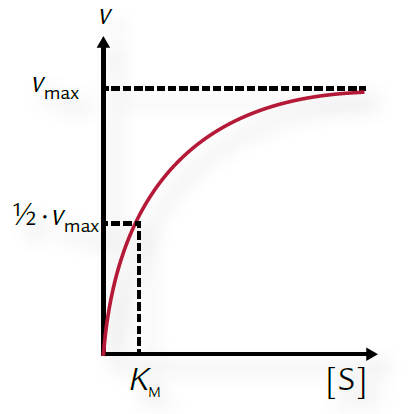
\includegraphics[scale=0.6]{Figurer/MMplot1} \hspace{2cm}
    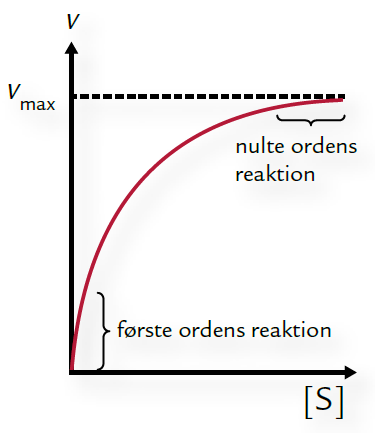
\includegraphics[scale=0.6]{Figurer/MMplot2}
    \caption{Michalis-Menten plot}
\end{figure}
På den ene figur ses den vigtige obeservartion at når $K_M=[S]$ da er $v=\frac{1}{2}v_{max}$.
På den anden figur ses at ved meget lille koncentraton af substrat, der opfører reaktionen sig tilnærmelsesvist som om at den var af første orden mht. substratkoncentrationen. 
Det ses også at ved stor koncentration opfører den sig næsten som om at den var af 0'te orden.